\documentclass[a4paper, 10pt, ]{article}

\input{./COMMONFILES/preamble.tex}

% -----------------------------------------------------------------------------

\def\oznacenieCelku{Kolekcia učebných textov}

% -----------------------------------------------------------------------------


\def\KUTporadoveCislo{dev250820}

\def\oznacenieVerzie{v0.9}
% \def\oznacenieVerzie{\phantom{v1.0}}

\def\mesiacRok{august 2025}

\def\authorslabel{MT}






% -----------------------------------------------------------------------------

\begin{document}

% -----------------------------------------------------------------------------
% Uvodny nadpis

\noindent
\parbox[t][18mm][c]{0.3\textwidth}{%
\raisebox{-0.9\height}{%
\phantom{.}\includegraphics[height=18mm]{./COMMONFILES/URKFEIlogo.pdf}%
}%
}%
\parbox[t][18mm][c]{0.7\textwidth}{%
\raggedleft

\sffamily
\fontsize{16pt}{18pt}
\fontseries{sbc}
\selectfont

\noindent
\textcolor[rgb]{0.75, 0.75, 0.75}{\textls[25]{\oznacenieCelku}}
}%

\noindent
\parbox[t][16mm][b]{0.5\textwidth}{%
\raggedright

\color{Gray}
\sffamily

\fontsize{12pt}{12pt}
\selectfont
\mesiacRok

\fontsize{6pt}{10pt}
\selectfont
\href{https://github.com/OkoliePracovnehoBodu/KUT}{github.com/OkoliePracovnehoBodu/KUT}

\fontsize{8pt}{10pt}
\selectfont
\authorslabel




}%
\parbox[t][16mm][b]{0.5\textwidth}{%
\raggedleft

\sffamily

\fontsize{6pt}{6pt}
\selectfont

\textcolor[rgb]{0.68, 0.68, 0.68}{\oznacenieVerzie}


\fontsize{14pt}{14pt}
\selectfont

\bfseries

\includegraphics[height=12pt]{./COMMONFILES/KUT_logo_v0.1.pdf}%
{%
\textls[-50]{\KUTporadoveCislo}
}%
}%

% -----------------------------------------------------------------------------




\vspace{6mm}

% ---------------------------------------------
\sffamily
\bfseries
\fontsize{18pt}{21pt}
\selectfont

\begin{flushleft}
    Laboratórne zariadenie TS:\\ orientačný prehľad
\end{flushleft}

\bigskip

% -----------------------------------------------------------------------------
\normalsize
\normalfont
% -----------------------------------------------------------------------------

\lstset{style=mystyle}










\noindent
\lettrine[lines=1, nindent=1pt, loversize=0.0]{C}{ieľom} 
textu je opis laboratórneho zariadenia TS predstavujúceho fyzický model spojitého dynamického systému.


\section{Opis dynamického systému}

TS, skratka od \emph{tepelný systém} (thermal system), je laboratórne zariadenie predstavujúce reálny dynamický systém. Pozostáva zo sklenenej trubice umiestnenej na podstave. Na jednom konci trubice je upevnený ventilátor, ktorý do trubice vháňa vzduch. V trubici hneď za ventilátorom sa nachádza výhrevné teleso (výhrevná špirála). Za špirálou je umiestnený prvý teplotný snímač a druhý je umiestnený na opačnom konci trubice. V~podstave sa nachádza elektronika zabezpečujúca napájanie komponentov zariadenia a~rozhranie k meracej karte.

Dostupnými sú dva vstupné a dva výstupné analógové signály. Prvý vstupný signál ovláda výkon vyhrievacieho telesa. Druhý vstupný signál ovláda výkon ventilátora. Prvý výstupný signál je teplota vzduchu v~trubici hneď za vyhrievacím telesom. Druhý výstupný signál je teplota vzduchu v trubici na opačnom konci od vyhrievacieho telesa.

Z kybernetického hľadiska je zariadenie TS možné prevádzkovať ako mnohovstupový a~mnohovýstupový systém (MIMO systém) alebo ako jednovstupový a jedno výstupový systém (SISO systém). 

Pri SISO systéme je vstupom signál ovládajúci výkon vyhrievacieho telesa. Signál pre ventilátor v podstate určuje prevádzkovú podmienku alebo prevádzkové nastavenie zariadenia keďže prúdenie vzduchu v trubici vo všeobecnosti vplýva na jeho ohrievanie a teplotu.





\section{Rozsahy a jednotky signálov}

Z opisu predmetného dynamického systému plynie, že systém ma dva vstupné a dva výstupné signály.

Všetky štyri signály nadobúdajú hodnoty v~rozsahu $0$ až $10$ pričom ide o~napäťové signály vo voltoch [V].

Signál ovládajúci výkon vyhrievacieho telesa označme vstup~1~a~signál ovládajúci výkon ventilátora označme vstup~2. Signál zo snímača teploty hneď za vyhrievacím telesom označme výstup~1 a~signál zo snímača teploty na opačnom konci trubice označme výstup~2.

\begin{center}

\vspace{-10pt}    
    
\tabcaption{Rozsahy a jednotky signálov}
\label{tab:rozsahy_a_jednotky_signalu}

\lstyle

\begin{tabular*}{\textwidth}{@{ \extracolsep{\fill}} lll}
\toprule
Signál & Rozsah hodnôt & Jednotka \\
\midrule
Vstup 1 & $0$ až $10$ & V (volt) \\
Vstup 2 & $0$ až $10$ & V (volt) \\
Výstup 1 & $0$ až $10$ & V (volt) \\
Výstup 2 & $0$ až $10$ & V (volt) \\
\bottomrule
\end{tabular*}


\end{center}













\section{Schematické znázornenie systému}


\begin{center}

    \vbox{%


        \makebox[\textwidth][c]{%
        \includegraphics{TS_sch1.pdf}
        }

        \figcaption{ 
            Signály systému TS.
        }
        \label{TS_sch1}
    }%vbox

\end{center}


\begin{center}

    \vbox{%


        \makebox[\textwidth][c]{%
        \includegraphics{TS_sch2b.pdf}
        }

        \figcaption{ 
            Schéma pripojenia laboratórneho zariadenia k svorkám meracej karty Advantech PCI-1711, pričom AO~$0$ a AO~$1$ sú analógové výstupy meracej karty a~AI~$0$, AI~$1$ sú analógové vstupy meracej karty.
        }
        \label{TS_sch2b}
    }%vbox

\end{center}



\section{Fotografie}

Zoznam fotografií:

\begin{itemize}[leftmargin=0pt, labelsep=3mm, itemsep=0pt]
    \item Obr. \ref{IMG_5575_toPDF}: Celkový pohľad na laboratórne zariadenie TS.
    \item Obr. \ref{IMG_5589_toPDF}: Detail na sklenenú trubicu laboratórneho zariadenia TS.
    \item Obr. \ref{TS_sch3_foto}: Pohľad zhora s vyznačením jednotlivých komponentov.   
\end{itemize}

\noindent
\vbox{%

    \makebox[\textwidth][c]{%
    \includegraphics{IMG_5575_toPDF.jpg}
    }

    \figcaption{ 
        Celkový pohľad na laboratórne zariadenie TS.
    }
    \label{IMG_5575_toPDF}
}%vbox

\vfill

\noindent
\vbox{%

    \makebox[\textwidth][c]{%
    \includegraphics{IMG_5589_toPDF.jpg}
    }

    \figcaption{ 
        Detail na sklenenú trubicu laboratórneho zariadenia TS. 
    }
    \label{IMG_5589_toPDF}
}%vbox


\bigskip

\noindent
\vbox{%

    \makebox[\textwidth][c]{%
    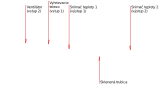
\includegraphics{TS_sch3_foto.pdf}
    }

    \figcaption{ 
        Pohľad zhora s vyznačením jednotlivých komponentov. 
    }
    \label{TS_sch3_foto}
}%vbox

































































% -----------------------------------------------------------------------------

\end{document}

% -----------------------------------------------------------------------------